%
% vektorprodukt.tex
%
% (c) 2018 Prof Dr Andreas Müller, Hochschule Rapperswil
%
\section{Orientierung}
\rhead{Orientierung}
Mit dem Skalarprodukt haben wir ein Werkzeug, Längen und Winkel zu berechnen,
es fehlt jedoch noch ein Werkzeug, Volumina einfach zu berechnen.
Orthonormierte
Vektorsysteme haben wir als sehr nützlich erkannt, aber die Bestimmung eines
Vektors, der auf zwei gegebenen Vektoren senkrecht steht, ist eher kompliziert.
Uns stand bislang entweder das
aufwendige Orthogonalisierungsverfahren zur Verfügung, oder die Lösung
eines Gleichungssystems mit dem Gauss-Algorithmus.

Dabei haben wir im Kapitel \ref{chapter-determinanten} bereits alles
bereitgestellt, was wir für die Volumenberechnung benötigen.
Wir werden auf diesem Weg eine neue Vektoroperation kennenlernen,
das Vektorprodukt.

\subsection{Flächeninhalt eines Parallelogramms}
\begin{figure}
\begin{center}
%\includegraphics{images/d-1}
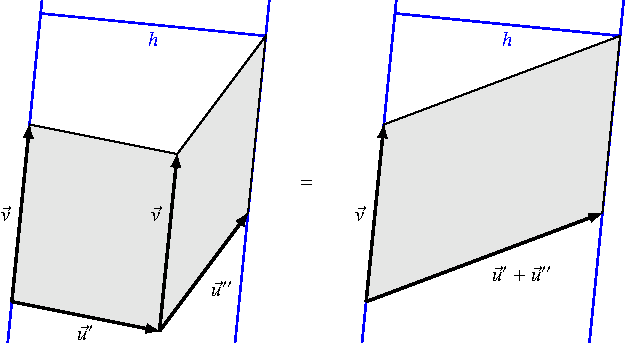
\includegraphics{5/images/flaeche.pdf}
\end{center}
\caption{Addition von Flächeninhalten von Parallelogrammen.
Beide Flächen haben die gleiche Grundseite $|\vec{v}|$ und die gleiche
Höhe $h$, also ist der graue Flächeninhalt beider Figuren gleich.
Daraus lässt sich ableiten, dass der orientierte Flächeninhalt linear
ist in jedem Argument.
\label{image-flaeche-addition}}
\end{figure}
Zwei Vektoren $\vec u$ und $\vec v$ spannen in der Ebene ein Parallelogramm
auf.
Gesucht ist der Flächeninhalt des Parallelogramms.
Statt dafür eine
Formel abzuleiten, untersuchen wir zunächst die Eigenschaften dieses
Flächeninhaltes in der Hoffnung, dass wir bereits ein Objekt mit den
gleichen Eigenschaften kennen.

Wir bezeichnen den Flächeninhalt des von $\vec u$ und $\vec v$ aufgespannten
Parallelogramms mit $A(\vec u,\vec v)$.
Der Flächeninhalt im landläufigen
Sinne ist natürlich immer positiv, es stellt sich jedoch als
zweckmässig heraus, wenn wir den Flächeninhalt hier mit einem
Vorzeichen versehen.
Und zwar soll $A(\vec u,\vec v)$ positiv sein, wenn
sich $\vec u$ mit einer Drehung von weniger als $180^\circ$ in den Vektor
$\vec v$ drehen lässt.
Wir nennen $A(\vec u, \vec v)$ den orientierten
Flächeninhalt.

Die Funktion $A(\vec u,\vec v)$ hat folgende Eigenschaften
\begin{itemize}
\item $A$ ändert das Vorzeichen bei Vertauschung der beiden Vektoren.
\item $A$ ist linear im ersten Argument:
\begin{align*}
A(\vec u'+\vec u'',\vec v)&=A(\vec u',\vec v)+A(\vec v'',\vec u)
\\
A(\lambda \vec u,\vec v)&=\lambda A(\vec u,\vec v)
\end{align*}
\item Der Flächeninhalt eines Einheitsquadrates ist $A(\vec e_1,\vec e_2)=1$.
\end{itemize}
Die beiden Eigenschaften zusammen ergeben, dass $A$ auch linear im
zweiten Argument ist.
Im Kapitel~2 haben wir gelernt, dass es nur eine
Funktion mit diesen Eigenschaften gibt, nämlich die Determinante:
\begin{satz}
Der orientierte Flächeninhalt des von den Vektoren $\vec u$ und $\vec v$
aufgespannten Parallelogramms ist
\[
A(\vec u,\vec v)=\left|\;\begin{matrix}u_1&v_1\\u_2&v_2\end{matrix}\;\right|
=u_1v_2-u_2v_1
.
\]
\end{satz}
\begin{satz}
Der Flächeninhalt eines Dreiecks mit den Ecken $(x_1,y_1)$, $(x_2,y_2)$ und
$(x_3,y_3)$ ist
\[
F=
\frac12\left|\;
\begin{matrix}
x_1-x_3&x_2-x_3\\
y_1-y_3&y_2-y_3\\
\end{matrix}
\;\right|
\]
\end{satz}

\begin{beispiel}
Man berechne den Flächeninhalt des Dreiecks mit den Ecken
$A=(1,6)$, $B=(7,5)$ und $C=(5,3)$.

\smallskip

{\parindent 0pt Die Kantenvektoren} des Dreiecks $ABC$ sind
\[
\overrightarrow{AB}=\begin{pmatrix}6\\-1\end{pmatrix}
,\qquad
\overrightarrow{AC}=\begin{pmatrix}4\\-3\end{pmatrix}
\]
und der Flächeninhalt
\[
F=\frac12\left|\;\begin{matrix}
   6&  4\\
  -1& -3
\end{matrix}\;\right|=
-7
.
\]
Der Flächeninhalt ist also $7$.
\end{beispiel}

\subsection{Volumen eines Parallelepipeds}
\begin{figure}
\begin{center}
%\includegraphics{images/d-2}
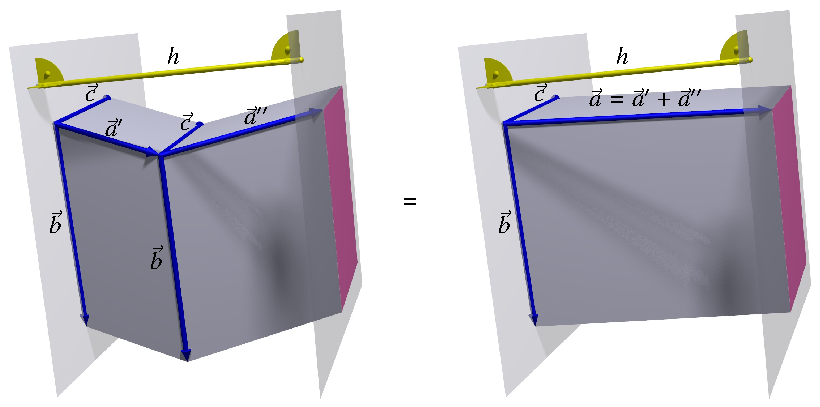
\includegraphics{5/images/volumen.pdf}
\end{center}
\caption{Addition der Volumina von Parallelepipeds.
Da die beiden Körper die gleiche Höhe und die gleiche (pinke) Grundfläche
haben, haben Sie auch das gleiche Volumen.
Daraus kann man ablesen, dass das orientierte Volumen linear ist.
\label{image-volumina}}
\end{figure}
Ganz ähnlich kann man das Volumen eines Parallelepipeds in drei Dimensionen
berechnen, welches von drei Vektoren $\vec a$, $\vec b$ und $\vec c$
aufgespannt wird.
Auch hier stellt es sich als nützlich heraus,
das Volumen mit einem Vorzeichen zu versehen:
\begin{definition}
Das orientierte Volumen
$V(\vec a,\vec b,\vec c)$
eines Parallelepipeds aufgespannt von den drei
Vektoren
$\vec a$, $\vec b$ und $\vec c$ ist positiv, wenn die drei Vektoren
eine ``rechtshändiges System'' bilden, also gegeneinander orientiert
sind wie die ersten drei Finger der rechten Hand, andernfalls ist
$V(\vec a,\vec b,\vec c)$ negativ.
\end{definition}
Dieses orientierte Volumen hat die folgenden Eigenschaften:
\begin{enumerate}
\item Vertauscht man zwei der drei Vektoren, ändert das Volumen das Vorzeichen.
\item $V(\vec a,\vec b,\vec c)$ ist linear im ersten Argument, wie man
der Abbildung~\ref{image-volumina} entnehmen kann:
\begin{align*}
V(\lambda\vec a,\vec b,\vec c)
&=
\lambda V(\vec a,\vec b,\vec c)
\\
V(\vec a'+\vec a'',\vec b,\vec c)
&=
V(\vec a',\vec b,\vec c)
+
V(\vec a'',\vec b,\vec c)
\end{align*}
\item Das orientierte Volumen des Einheitswürfels ist
$V(\vec e_1,\vec e_2,\vec e_3)=1$.
\end{enumerate}
Aus den ersten beiden Eigenschaften können wir folgern, dass das orientierte
Volumen auch in allen anderen Argumenten linear ist.
Und wie im vorangegangenen Abschnitt schliessen wir,
dass $V(\vec a,\vec b,\vec c)$ die Determinante ist:
\begin{satz}
Das orientierte Volumen $V(\vec a,\vec b,\vec c)$ eines von den Vektoren
$\vec a$, $\vec b$ und $\vec c$ aufgespannten Parallepipeds  ist
\[
V(\vec a,\vec b,\vec c)=\left|\;\begin{matrix}
a_1&b_1&c_1\\
a_2&b_2&c_2\\
a_3&b_3&c_3\\
\end{matrix}\;\right|.
\]
\end{satz}
\begin{figure}
\centering
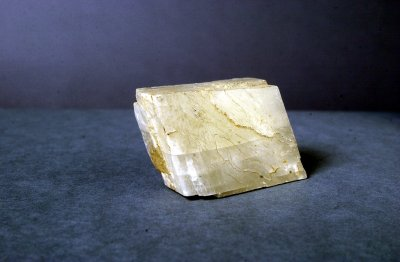
\includegraphics[width=0.7\hsize]{graphics/calcite.jpg}
\caption{Ein Kalzit- oder Kalkspat-Kristall hat die Form eines Parallelepipeds.
Minerale, die sich gut spalten lassen, werden in der Geologie als Spate
bezeichnet, die Spaltprodukte sind angenäherte Parallelepipeds.
\label{skript:orientierung:calcite}}
\end{figure}
Das Parallelepiped wird auch als {\em Spat} bezeichnet.
In der Geologie werden gut spaltbare Minerale als Spate bezeichnet, zum
Beispiel Feldspat oder Kalkspat (Abbildung~\ref{skript:orientierung:calcite}.)
Durch Spaltung gewonnene Kristalle dieser Minerale sind gute Approximationen
von Parallelepipeds.
Das Volumen $V(\vec{a},\vec{b},\vec{c})$ des von $\vec{a}$, $\vec{b}$ und
$\vec{c}$ aufgespannten Parallelepipeds heisst daher auch das Spatvolumen.

\begin{beispiel}
Man finde alle Parallelepipeds mit folgenden Eigenschaften:
\begin{compactenum}
\item Zwei Kanten sind $\vec a=\overrightarrow{OA}$ und $\vec b=\overrightarrow{OB}$
mit $A=(4,1,3)$ und $B=(5,1,2)$.
\item Die dritte Kante ist $\overrightarrow{OC}$, wobei $C$ auf der
Ebene durch $O$ mit der Normalen
\[
\vec n=\begin{pmatrix}1\\1\\1\end{pmatrix}
\]
liegt.
\item Zwei Kanten stehen senkrecht aufeinander.
\item Das Volumen ist $8$.
\end{compactenum}

\smallskip

{\parindent 0pt Wir suchen einen Vektor}
\[
\vec c=\begin{pmatrix}x\\y\\z\end{pmatrix},
\]
der die Bedingungen der Aufgabe erfüllt.
Zunächst muss $\vec c$ auf $\vec n$ senkrecht stehen,
also $\vec c\cdot\vec n=0$ oder
\[
x+y+z=0.
\]
Da $\vec a\cdot\vec b=20+1+6=27\ne 0$ stehen $\vec a$ und $\vec b$
nicht senkrecht, es ist also der gesuchte Vektor $\vec c$ der auf den bereits
bekannten Kanten senkrecht stehen muss.
Wir versuchen es zunächst
mit $\vec a$, weitere Lösungen ergeben sich, wenn man stattdessen $\vec b$
verwendet.
Dies liefert die Bedingung $\vec a\cdot\vec c=0$ oder
\[
4x+y+3z=0
\]
Das Volumen kann mit der Determinante berechnet werden:
\[
V=\left|\;
\begin{matrix}
4&5&x\\
1&1&y\\
3&2&z
\end{matrix}
\;\right|=
4z+15y+2x-3x-8y-5z=-x+7y-z=\pm8.
\]
Jetzt kann der Vektor $\vec c$ mit dem Gauss-Algorithmus bestimmt werden
\begin{align*}
\begin{tabular}{|>{$}c<{$}>{$}c<{$}>{$}c<{$}|>{$}c<{$}|}
\hline
1%
\begin{picture}(0,0)
\color{red}\put(-3,4){\circle{12}}
\end{picture}%
&1&1&0\\
-1&7&-1&\pm8\\
4%
\begin{picture}(0,0)%
\color{blue}\drawline(-12,-2)(-12,24)(4,24)(4,-2)
\end{picture}%
&1&3&0\\
\hline
\end{tabular}
&
\rightarrow
\begin{tabular}{|>{$}c<{$}>{$}c<{$}>{$}c<{$}|>{$}c<{$}|}
\hline
1&1&1&0\\
0&8%
\begin{picture}(0,0)
\color{red}\put(-3,4){\circle{12}}
\end{picture}%
&0&\pm8\\
0&-3%
\begin{picture}(0,0)%
\color{blue}\drawline(-15,-2)(-15,10)(1,10)(1,-2)
\end{picture}%
&-1&0\\
\hline
\end{tabular}
\rightarrow
\begin{tabular}{|>{$}c<{$}>{$}c<{$}>{$}c<{$}|>{$}c<{$}|}
\hline
1&1&1&0\\
0&1&0%
\begin{picture}(0,0)%
\color{blue}\drawline(-8,24)(-8,-2)(2,-2)(2,24)
\end{picture}%
&\pm1\\
0&0&-1%
\begin{picture}(0,0)
\color{red}\put(-7,4){\circle{15}}
\end{picture}%
&\pm3\\
\hline
\end{tabular}
\\
&
\rightarrow
\begin{tabular}{|>{$}c<{$}>{$}c<{$}>{$}c<{$}|>{$}c<{$}|}
\hline
1&1%
\begin{picture}(0,0)%
\color{blue}\drawline(-8,10)(-8,-2)(2,-2)(2,10)
\end{picture}%
&0&\pm3\\
0&1&0&\pm1\\
0&0&1&\mp3\\
\hline
\end{tabular}
\rightarrow
\begin{tabular}{|>{$}c<{$}>{$}c<{$}>{$}c<{$}|>{$}c<{$}|}
\hline
1&0&0&\pm 2\\
0&1&0&\pm1\\
0&0&1&\mp3\\
\hline
\end{tabular}
\end{align*}
Es folgt $C=(\pm 2,\pm1,\mp3)$.
Zwei weitere Lösungen findet
man auf die gleiche Weise, indem man statt der Bedingung $\vec a\cdot\vec c=0$
verlangt, dass $\vec b\cdot\vec c=0$, man findet dann
\begin{align*}
\begin{tabular}{|>{$}c<{$}>{$}c<{$}>{$}c<{$}|>{$}c<{$}|}
\hline
1%
\begin{picture}(0,0)
\color{red}\put(-3,4){\circle{12}}
\end{picture}%
&1&1&0\\
-1&7&-1&\pm8\\
5%
\begin{picture}(0,0)%
\color{blue}\drawline(-12,-2)(-12,24)(4,24)(4,-2)
\end{picture}%
&1&2&0\\
\hline
\end{tabular}
&
\rightarrow
\begin{tabular}{|>{$}c<{$}>{$}c<{$}>{$}c<{$}|>{$}c<{$}|}
\hline
1&1&1&0\\
0&8%
\begin{picture}(0,0)
\color{red}\put(-3,4){\circle{12}}
\end{picture}%
&0&\pm8\\
0&-4%
\begin{picture}(0,0)%
\color{blue}\drawline(-15,-2)(-15,10)(1,10)(1,-2)
\end{picture}%
&-3&0\\
\hline
\end{tabular}
\rightarrow
\begin{tabular}{|>{$}c<{$}>{$}c<{$}>{$}c<{$}|>{$}c<{$}|}
\hline
1&1&1&0\\
0&1&0%
\begin{picture}(0,0)
\color{blue}\drawline(-8,24)(-8,-2)(2,-2)(2,24)
\end{picture}%
&\pm1\\
0&0&-3%
\begin{picture}(0,0)
\color{red}\put(-7,4){\circle{15}}
\end{picture}%
&\pm4\\
\hline
\end{tabular}
\\
&
\rightarrow
\begin{tabular}{|>{$}c<{$}>{$}c<{$}>{$}c<{$}|>{$}c<{$}|}
\hline
1&1%
\begin{picture}(0,0)
\color{blue}\drawline(-8,10)(-8,-2)(2,-2)(2,10)
\end{picture}%
&0&\pm\frac43\\
0&1&0&\pm1\\
0&0&1&\mp\frac43\\
\hline
\end{tabular}
\rightarrow
\begin{tabular}{|>{$}c<{$}>{$}c<{$}>{$}c<{$}|>{$}c<{$}|}
\hline
1&0&0&\pm\frac13\\
0&1&0&\pm1\\
0&0&1&\mp\frac43\\
\hline
\end{tabular}
\end{align*}
also
$C=(\pm\frac13,\pm1,\mp\frac43)$.
\end{beispiel}

